\documentclass[final,hyperref={pdfpagelabels=false}]{beamer}

\mode<presentation>{\usetheme{I6pd2_hugo}}
\usepackage[english]{babel}
\usepackage[latin1]{inputenc}
\usepackage{amsmath,amsthm, amssymb, latexsym, subfigure}
%\usepackage{times}\usefonttheme{professionalfonts}  % obsolete
%\usefonttheme[onlymath]{serif}
\boldmath
\usepackage[orientation=portrait,size=a0,scale=1.4,debug]{beamerposter}
% change list indention level
% \setdefaultleftmargin{3em}{}{}{}{}{}
\usecaptiontemplate{
\small
\structure{\insertcaptionname~\insertcaptionnumber:}
\insertcaption
}


%\usepackage{snapshot} % will write a .dep file with all dependencies, allows for easy bundling

\usepackage{array,booktabs,tabularx,subfigure,graphicx}
\newcolumntype{Z}{>{\centering\arraybackslash}X} % centered tabularx columns
\newcommand{\pphantom}{\textcolor{ta3aluminium}} % phantom introduces a vertical space in p formatted table columns??!!

\listfiles

%%%%%%%%%%%%%%%%%%%%%%%%%%%%%%%%%%%%%%%%%%%%%%%%%%%%%%%%%%%%%%%%%%%%%%%%%%%%%%%%%%%%%%
 
\title{Improvements to the LHC Injection Kickers Beam Screen}
\author{H. Day\thanks{hugo.day@hep.manchester.ac.uk}$^{\dagger}$, M.J. Barnes$^{\dagger}$, F. Caspers$^{\dagger}$, E. Metral$^{\dagger}$, B. Salvant$^{\dagger}$ \\
$\dagger$ CERN, Switzerland \\}
\date[May 23rd, 2011]{May 23rd, 2011}

%%%%%%%%%%%%%%%%%%%%%%%%%%%%%%%%%%%%%%%%%%%%%%%%%%%%%%%%%%%%%%%%%%%%%%%%%%%%%%%%%%%%%%
\newlength{\columnheight}
\setlength{\columnheight}{105cm}


%%%%%%%%%%%%%%%%%%%%%%%%%%%%%%%%%%%%%%%%%%%%%%%%%%%%%%%%%%%%%%%%%%%%%%%%%%%%%%%%%%%%%%
\begin{document}
\begin{frame}
  \begin{columns}
    % ---------------------------------------------------------%
    % Set up a column 
    \begin{column}{.49\textwidth}
      \begin{beamercolorbox}[center,wd=\textwidth]{postercolumn}
        \begin{minipage}[T]{.95\textwidth}  % tweaks the width, makes a new \textwidth
          \parbox[t][\columnheight]{\textwidth}{ % must be some better way to set the the height, width and textwidth simultaneously
            % Since all columns are the same length, it is all nice and tidy.  You have to get the height empirically
            % ---------------------------------------------------------%
            % fill each column with content            
            \begin{block}{Abstract}
\small{
The LHC injection kicker magnets (MKIs) experienced strong heating during the initial operation of the LHC up until the beginning of LS1 in 2013, sometimes necessitating cooling periods of 2-3 hours between fills. This heating was found to be caused by beam-induced heating due to beam-driven wakefields in the kicker magnets due to insufficient screening of the ferrite yoke by the beam screen within the yoke, originally necessitated due to concerns of HV breakdown on the beam screen. Recent studies proposed improvements to the beam screen which are to be implemented for LS1, which allows better screening of the ferrite yoke whilst improving HV behaviour. Further studies are under way to allow the MKIs to operate with HL-LHC parameters without experiencing negative effects due to beam-induced heating. Improvements to the resonant coaxial wire method, which permit greater frequency resolution, are also discussed.
}
\end{block}
            \vfill

	\begin{block}{LHC-MKI and Beam Screen Designs}

	\begin{itemize}
	\item{The MKIs have recently been observed to undergo significant temperature rise during the increase of the stored intensity in the LHC [1]. This has been confirmed to be due to beam-induced heating via interaction between the circulating beam and the beam-coupling impedance of the MKIs}
	\item{The beam-coupling impedance of the MKIs is dominated by the beam screen (see Fig.~\ref{fig:short-screens}); an alumina "carrier" tube into which are inserted a number of conductive strips.}

\begin{figure}
\includegraphics[width = 0.45\textwidth]{figures/shortening_screen_conductors.pdf}
\label{fig:short-screens}
\caption{Illustrating the layout of the beam screen, with the screen conductors electrically connected to the beam pipe at one end of the screen, and capacitively coupled to the beam pipe at the other by an overlapping external metallisation.}
\end{figure}

\item{Due to high voltage breakdown in the beam screen, most MKIs have had the 9 screen conductors closest to the HV plate removed. This causes an increase of the beam impedance, and thus increased heating.}

\begin{figure}
\subfigure[]{
\includegraphics[width = 0.45\textwidth]{figures/alternative_screen_design.pdf}
\label{fig:alt_screen}
}
\subfigure[]{
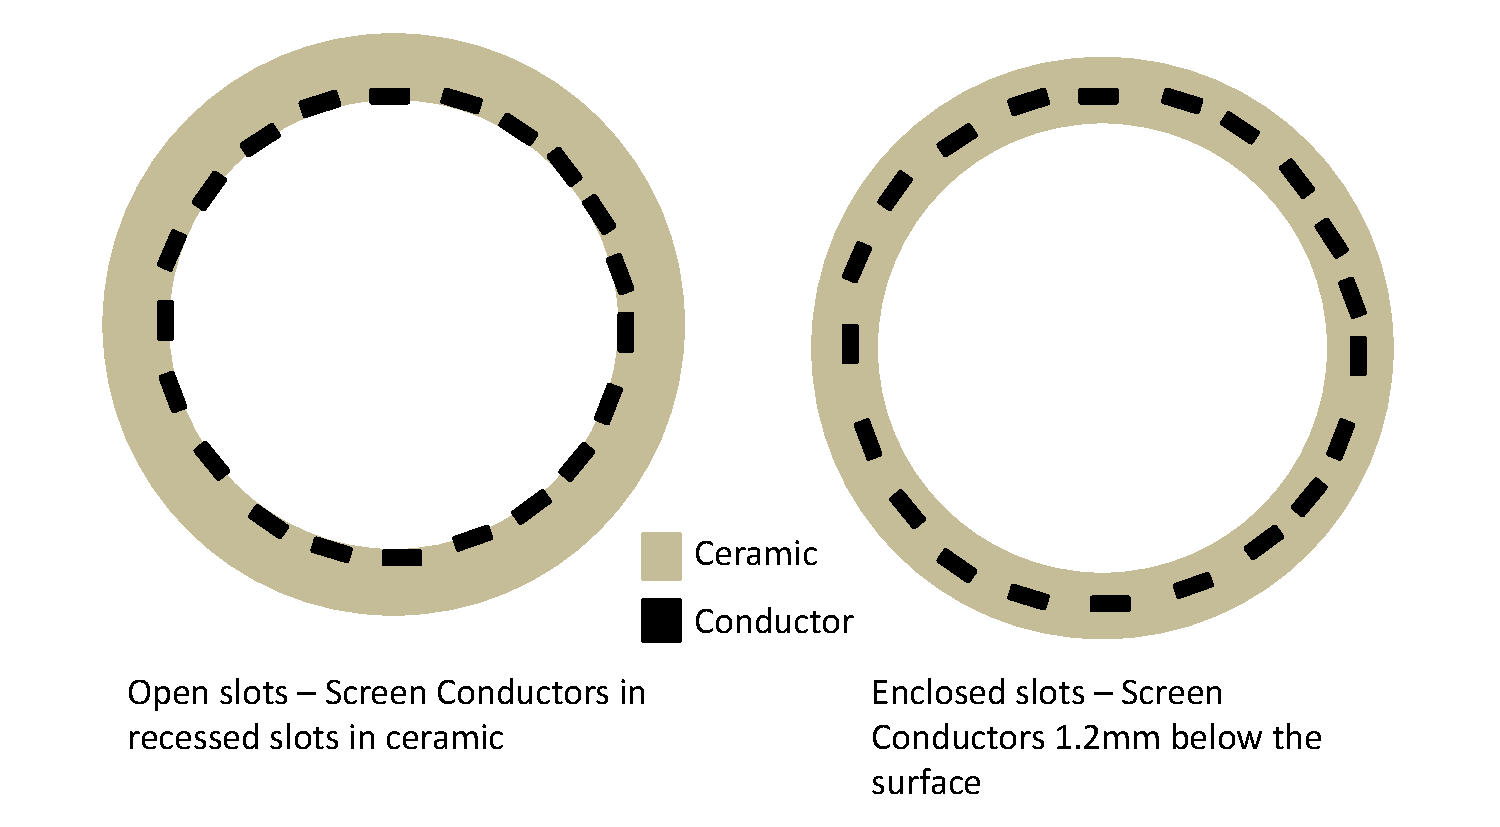
\includegraphics[width = 0.45\textwidth]{figures/enclosed_diagram.pdf}
\label{fig:enclosed_cond}
}
\label{fig:alternatives}
\caption{Cross sections of LHC-MKI beam screen with either \ref{fig:alt_screen} an alternative screen layout, in which most conductors are capactively coupled at both ends, and \ref{fig:enclosed_cond} the beam screen in which the screen conductors are in enclosed slots rather than open slots.}
\end{figure}
\item{A number of different beam screen configurations are considered to reduce the beam impedance and avoid electrical breakdown in the beam screen (see Fig.~2).}


	\end{itemize}
	\end{block}
 \vfill
\begin{block}{Simulations Parameters}

\begin{figure}
\includegraphics[width=0.8\linewidth]{figures/mki-cross-section.png}
\label{fig:kicker_xsec}
\caption{A cross section of the simulation model of the MKI. We see the transmission line kicker magnet structure with high voltage and ground plates, with capactive plates in between. In red we see the ferrite yolk, and damping ferrites at the end of the structure to damp $\lambda/4$ resonances of the screen conductors. The beam screen runs through the centre of the ferrite yoke.}
\end{figure}

\begin{itemize}
\item{The simulations of the beam coupling impedance of the MKI use a simplified model of the kicker magnet and vacuum tank (see Fig.~3), simulated interacting with a gaussian bunch of $\sigma_{z}=60mm$ in the time domain with the code CST Particle Studio. An integrated wake of 15m was used, using a mesh of $\approx$28 million cells.}

\end{itemize}

\end{block}
            \vfill

\begin{block}{References}
\small{1) \emph{"Analysis of Measured Ferrite Heating of the LHC Injection Kickers and Proposals for Future Reduction of Temperature"}, M.J. Barnes, L. Ducimetiere, N. Garrel. B. Goddard, W. Weterings, These proceedings}

\end{block}

           \vfill
         \vfill
          }
        \end{minipage}
      \end{beamercolorbox}
    \end{column}
    % ---------------------------------------------------------%
    % end the column

    % ---------------------------------------------------------%
    % Set up a column 
    \begin{column}{.49\textwidth}
      \begin{beamercolorbox}[center,wd=\textwidth]{postercolumn}
        \begin{minipage}[T]{.95\textwidth} % tweaks the width, makes a new \textwidth
          \parbox[t][\columnheight]{\textwidth}{ % must be some better way to set the the height, width and textwidth simultaneously
            % Since all columns are the same length, it is all nice and tidy.  You have to get the height empirically
            % ---------------------------------------------------------%
            % fill each column with content
\begin{block}{Coaxial Wire Measurements}
\begin{itemize}
\item{We compare measurements to simulations to verify the validity of the simulation model. We take the example of 15 screen conductors, which has existing measurement data (see Fig.~\ref{fig:meas_sim_comp}). We can see the agreement is very good over a substantial part of the frequency range considered.}
\end{itemize}
\begin{figure}
\includegraphics[width = 0.35\textwidth]{figures/15_conductors_meas_sims_ipac.pdf}
\caption{A comparison between the simulations and measurements of an LHC MKI with a beam screen with 15 screen conductors in open slots.}
\label{fig:meas_sim_comp}
\end{figure}


\end{block}
\vfill

\begin{block}{Beam Coupling Impedance of Beam Screen Designs}
\begin{itemize}
\item{Fig.~\ref{fig:screen_cond}(a) shows the impedance of the beam screen with different numbers of screen conductors. It can be seen that even a small amount of additional screening can contribute quite significantly to reducing the impedance of the MKI. The screening is especially effective at low frequencies where the beam current spectrum is high.}

\begin{figure} 
\subfigure[]{
\includegraphics[width=0.35\textwidth]{figures/15_24_conductors_near_hv_plate.pdf}
\label{fig:screen_cond}
}
\subfigure[]{
\includegraphics[width=0.35\textwidth]{figures/24_screens_different_designs.pdf}
\label{fig:new-screens}
}

\caption{The longitudinal beam coupling impedance of \ref{fig:screen_cond} different numbers of screen conductors in the beam screen of the MKI and \ref{fig:new-screens} different screen layouts for the MKI.}
\label{fig:screen_cond}
\end{figure}

\item{Fig.~\ref{fig:new-screens} shows the beam coupling impedance of a number of alternative screen designs compared to the present design with 24 screen conductors in place. We can see that all of these designs exhibit the same resonant structure, this being determined largely by the dimensions of the overlap between the screen conductors and the external metallisation. Work is underway to understand these resonances as a product of open-ended $\lambda/2$ resonators.}

\end{itemize}
\end{block}
\vfill

\begin{block}{Heating Estimates}
\begin{table}
\begin{center}
\caption{Estimates of the total power loss (Watts) due to the beam coupling impedance of an entire MKI for a number of different beam screen configurations and layouts. Estimates are given with two different bunch lengths. The alternative layout is that shown in Fig.~\ref{fig:alt_screen}. Thick ceramic indicates using a thicker ceramic (5.5mm thick as opposed to 4mm for all other designs).}
\begin{tabular*}{0.9\textwidth}{@{\extracolsep{\fill}} c | c | c | c | c }

 & \multicolumn{2}{|r|}{\footnotesize{Bunch Length $\sigma_{z} = 1.2ns$}} & \multicolumn{2}{|c}{\footnotesize{Bunch Length $\sigma_{z} = 1.3ns$}}\\ \hline
\small{Beam Screen Layout} & 25ns & 50ns & 25ns & 50ns \\ \hline
\footnotesize{No Beam Screen }& 4933&2784 &4320 & 2395\\ \hline
\footnotesize{24 Screen Conductors, open }&38 &13 &37 & 12\\ \hline
\footnotesize{15 Screen Conductors, open} &147 &72 &129 & 60\\ \hline
\footnotesize{24 Screen Conductors, enclosed} &76 &23 &73 & 22\\ \hline
\footnotesize{24 Screen Conductors, open, thick ceramic} &53 & 20&52 & 19\\ \hline
\footnotesize{24 Screen Conductors, open, alternative layout} &63 & 23&62 & 22\\ \hline
\footnotesize{19 Screen Conductors, open} &52 &18 &50 & 16\\ \hline
\footnotesize{20 Screen Conductors, open} &50 & 16& 48& 15\\ 
\end{tabular*}
\label{tab:power-loss}
\end{center}
\end{table}


\end{block}
\vfill
\begin{block}{Summary}
\begin{itemize}
\item{We have demonstrated a number of alternative beam screen designs for the LHC MKIs, in particular designs optimised to reduce electrical breakdown have been demonstrated to provide comparable heat loads as the original.}
\item{Using modern simulation tools it is possible to simulate very large and complex structures to produce results in good agreement with measurements.}
\end{itemize}
\end{block}
\vfill

          }
          % ---------------------------------------------------------%
          % end the column
        \end{minipage}
      \end{beamercolorbox}
    \end{column}
    % ---------------------------------------------------------%
    % end the column
  \end{columns}
  \vskip1ex
  %\tiny\hfill\textcolor{ta2gray}{Created with \LaTeX \texttt{beamerposter}  \url{http://www-i6.informatik.rwth-aachen.de/~dreuw/latexbeamerposter.php}}
%  \tiny\hfill{Created with \LaTeX \texttt{beamerposter}  \url{http://www-i6.informatik.rwth-aachen.de/~dreuw/latexbeamerposter.php} \hskip1em}
\end{frame}
\end{document}


%%%%%%%%%%%%%%%%%%%%%%%%%%%%%%%%%%%%%%%%%%%%%%%%%%%%%%%%%%%%%%%%%%%%%%%%%%%%%%%%%%%%%%%%%%%%%%%%%%%%
%%% Local Variables: 
%%% mode: latex
%%% TeX-PDF-mode: t
%%% End:
